% !TeX root = ../main.tex
% !TeX spelling = en_GB
% !TeX program = pdflatex

\chapter{Methods}
\label{chap:methods}

\section{Starting Studies}
Infrared and Visible Light
We describe the measured droplets as spherical lenses made of pure water at a constant temperature, surrounded by air. For simplicity we assume that the refractive index of air is equal to one.
\subsection{Laser Light}

\subsection{Image Noise}

\subsection{Light Sensitivity Measurement}

\subsection{Speed of Light Flash}

\section{Design Considerations}

We describe the measured droplets as spherical lenses made of pure water at a constant temperature, surrounded by air. For simplicity we assume that the refractive index of air is equal to one.

\subsection{Optics}

We assume that the optical silhouette of a droplet is comparable to a dot having equal diameter and being printed on a silicon glass. It is not a new concept and has at least once been proved experimentally for coherent light, by comparing with beads of glass and water droplets of known sizes (Korolev, Kuznetsov, Makarov, \& Novikov, 1991). The shadow image of water drops of any size will be defined mainly by the diffracted component, as long as the distance between the drop and the lens is much larger than the drop diameter. Only in a small bright spot in the middle will the refracted component be large enough to be visible in a shadowgraph system (Korolev et al., 1991; Wendisch \& Brenguier, 2013).



\section{The Shadowgraph System}

The system consists of a monochrome digital image sensor with a telecentric lens and a collimated LED illumination.

\begin{figure}%[h]
\centering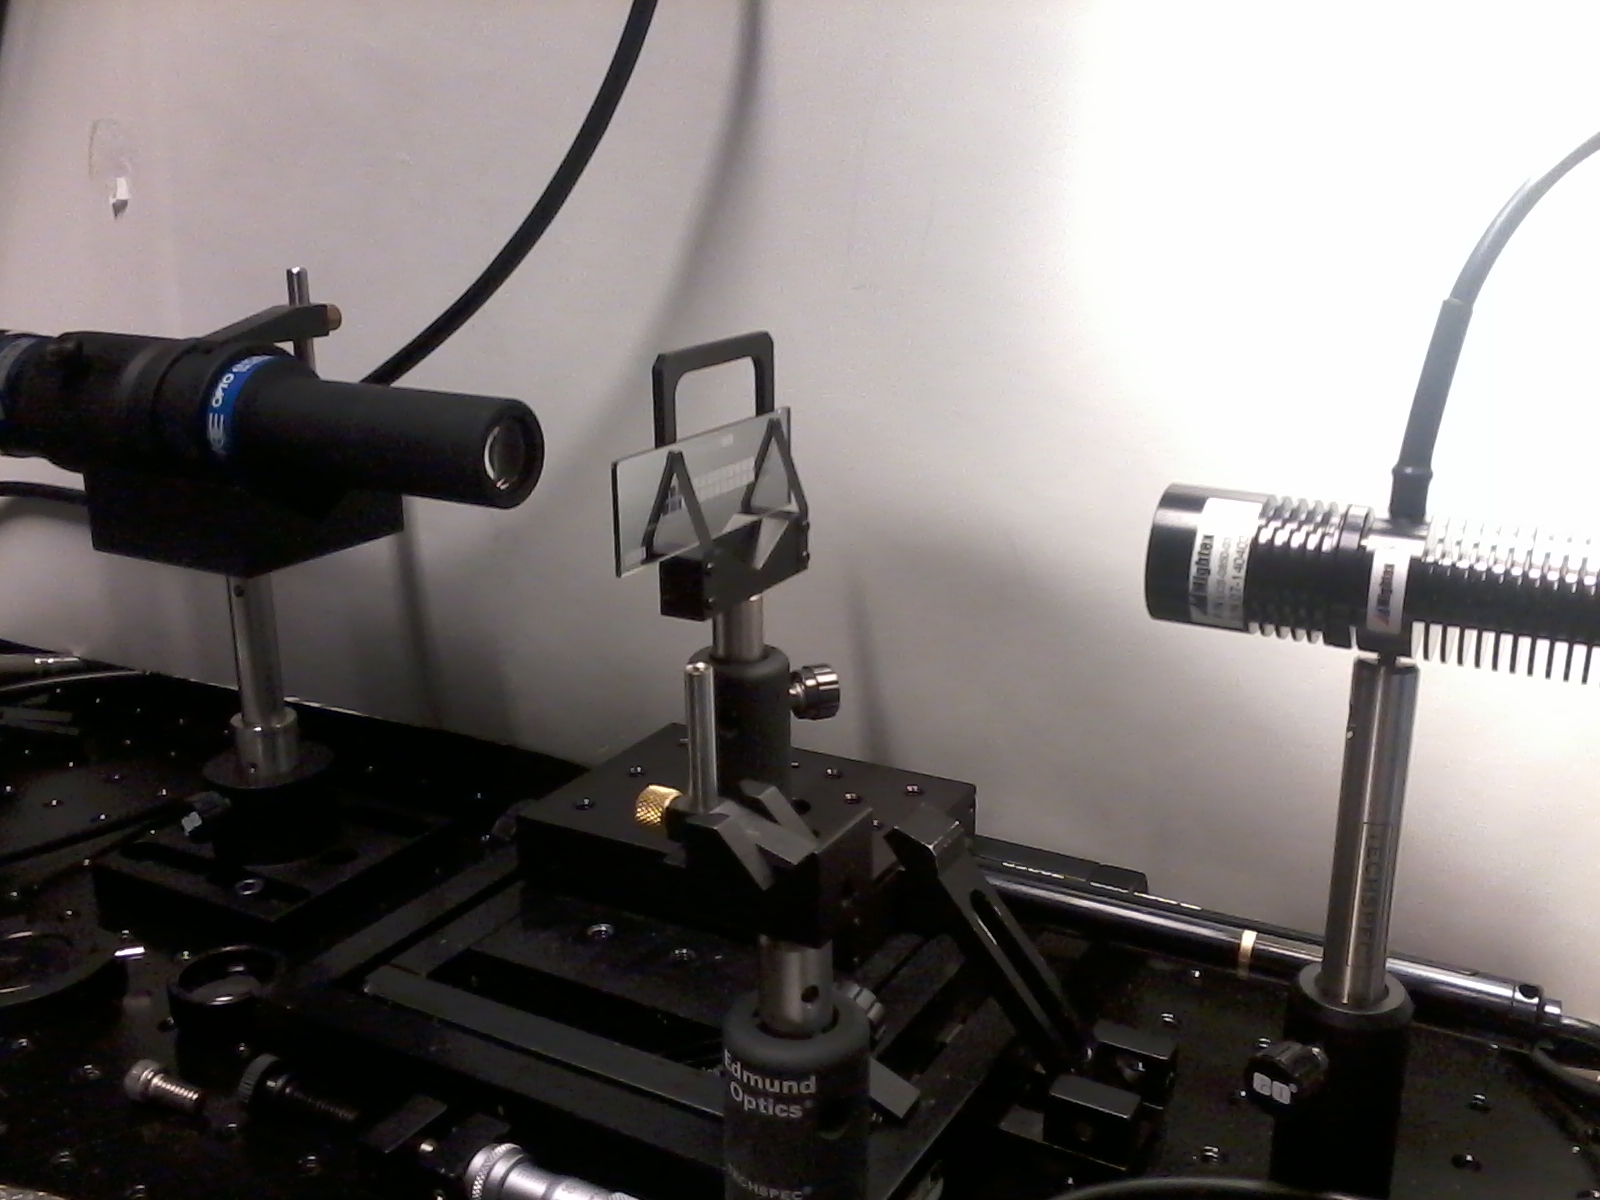
\includegraphics[width=0.6\linewidth]{figures/Foto0169}
\caption{Figure showing the experimental setup with a dot micrometer scale as test object mounted on a translation stage.}
\end{figure}

Calibration of true droplet size and measuring range both depends on the measured size of the droplet shadow and the amount of light used for exposure. It is possible to predict both the precision of the measured size and accuracy for measurement of droplet size. 

A value of both MVD and LWC can be derived from a series of images and since the number of measured droplets will depend on the concentration, the accuracy and precision will depend on the number of samples from the total population of droplets. 

Many existing instruments suffer from errors caused by the instrument itself during sampling, e.g. when droplets get stuck on the inlet [19], or shatters into smaller droplets [20]. An instrument should be designed in order to affect the free flow of particles as little as possible [16]. Therefore we also investigate the illuminative power required to get a good exposure with the tested system at a targeted maximum wind speed of 50 m/s.

We used a stage micrometer scale for characterization of the system and simulation of water droplets. This characterization holds true given that the optical silhouette of a droplet is comparable to a dot having equal diameter and being printed on a silicon glass. It is not a new concept and has at least once been proved experimentally for coherent light, by comparing with beads of glass and water droplets of known sizes [21]. The shadow image of water drops of any size will be defined mainly by the diffracted component, as long as the distance between the drop and the lens is much larger than the drop diameter. Only in a small bright spot in the middle will the refracted component be large enough to be visible. [21, 22]. 
Using the results of this study, a weather protected prototype may be built to perform a comparative study.


The design using a weakly collimated LED that illuminates an area slightly larger than the field of view makes the system quite insensitive to misalignment of the camera and the light source. Temporal or permanent changes in light intensity caused by a minor misalignment can be automatically compensated for by continuous measurement of the total exposure level. If the level of exposure is increasing or decreasing, the length of the light pulse is changed correspondingly. The light intensity can also be affected by dirt on the front glass of the housings. 

Spatial dissimilarities in the light intensity that are not caused by noise we can compensate for by calculating the local average intensity of the background around each measured droplet. The size of a droplet is then based on the intensity dip caused by the shadow compared with its local background.


making a flat-field correction. This is done by constructing an average image by the last 20 images and using this as a 


\section{The Fog Chamber}
The fog chamber is needed partly for practical reasons since natural fogs tend not to occur just when we are ready to test. It gives an indication of how the instrument will behave in a real measurement. It is also a verification of the instrument’s water ingress resistance. 
The chamber has a frame made of 30 mm aluminum profiles, fitted with transparent 6 mm polycarbonate walls on all sides using rubber sealing strips. The droplets are produced using an ultrasonic fog generator pushing the droplets to the chamber through a flexible tube approximately 30 mm in diameter and 500 mm long. Next to the fog inlet, there is a dry air inlet with a speed adjustable fan. See Fig. 7. On the back of the chamber there is a similar sized outlet for air and moisture.
 
\begin{figure}%[h]
\centering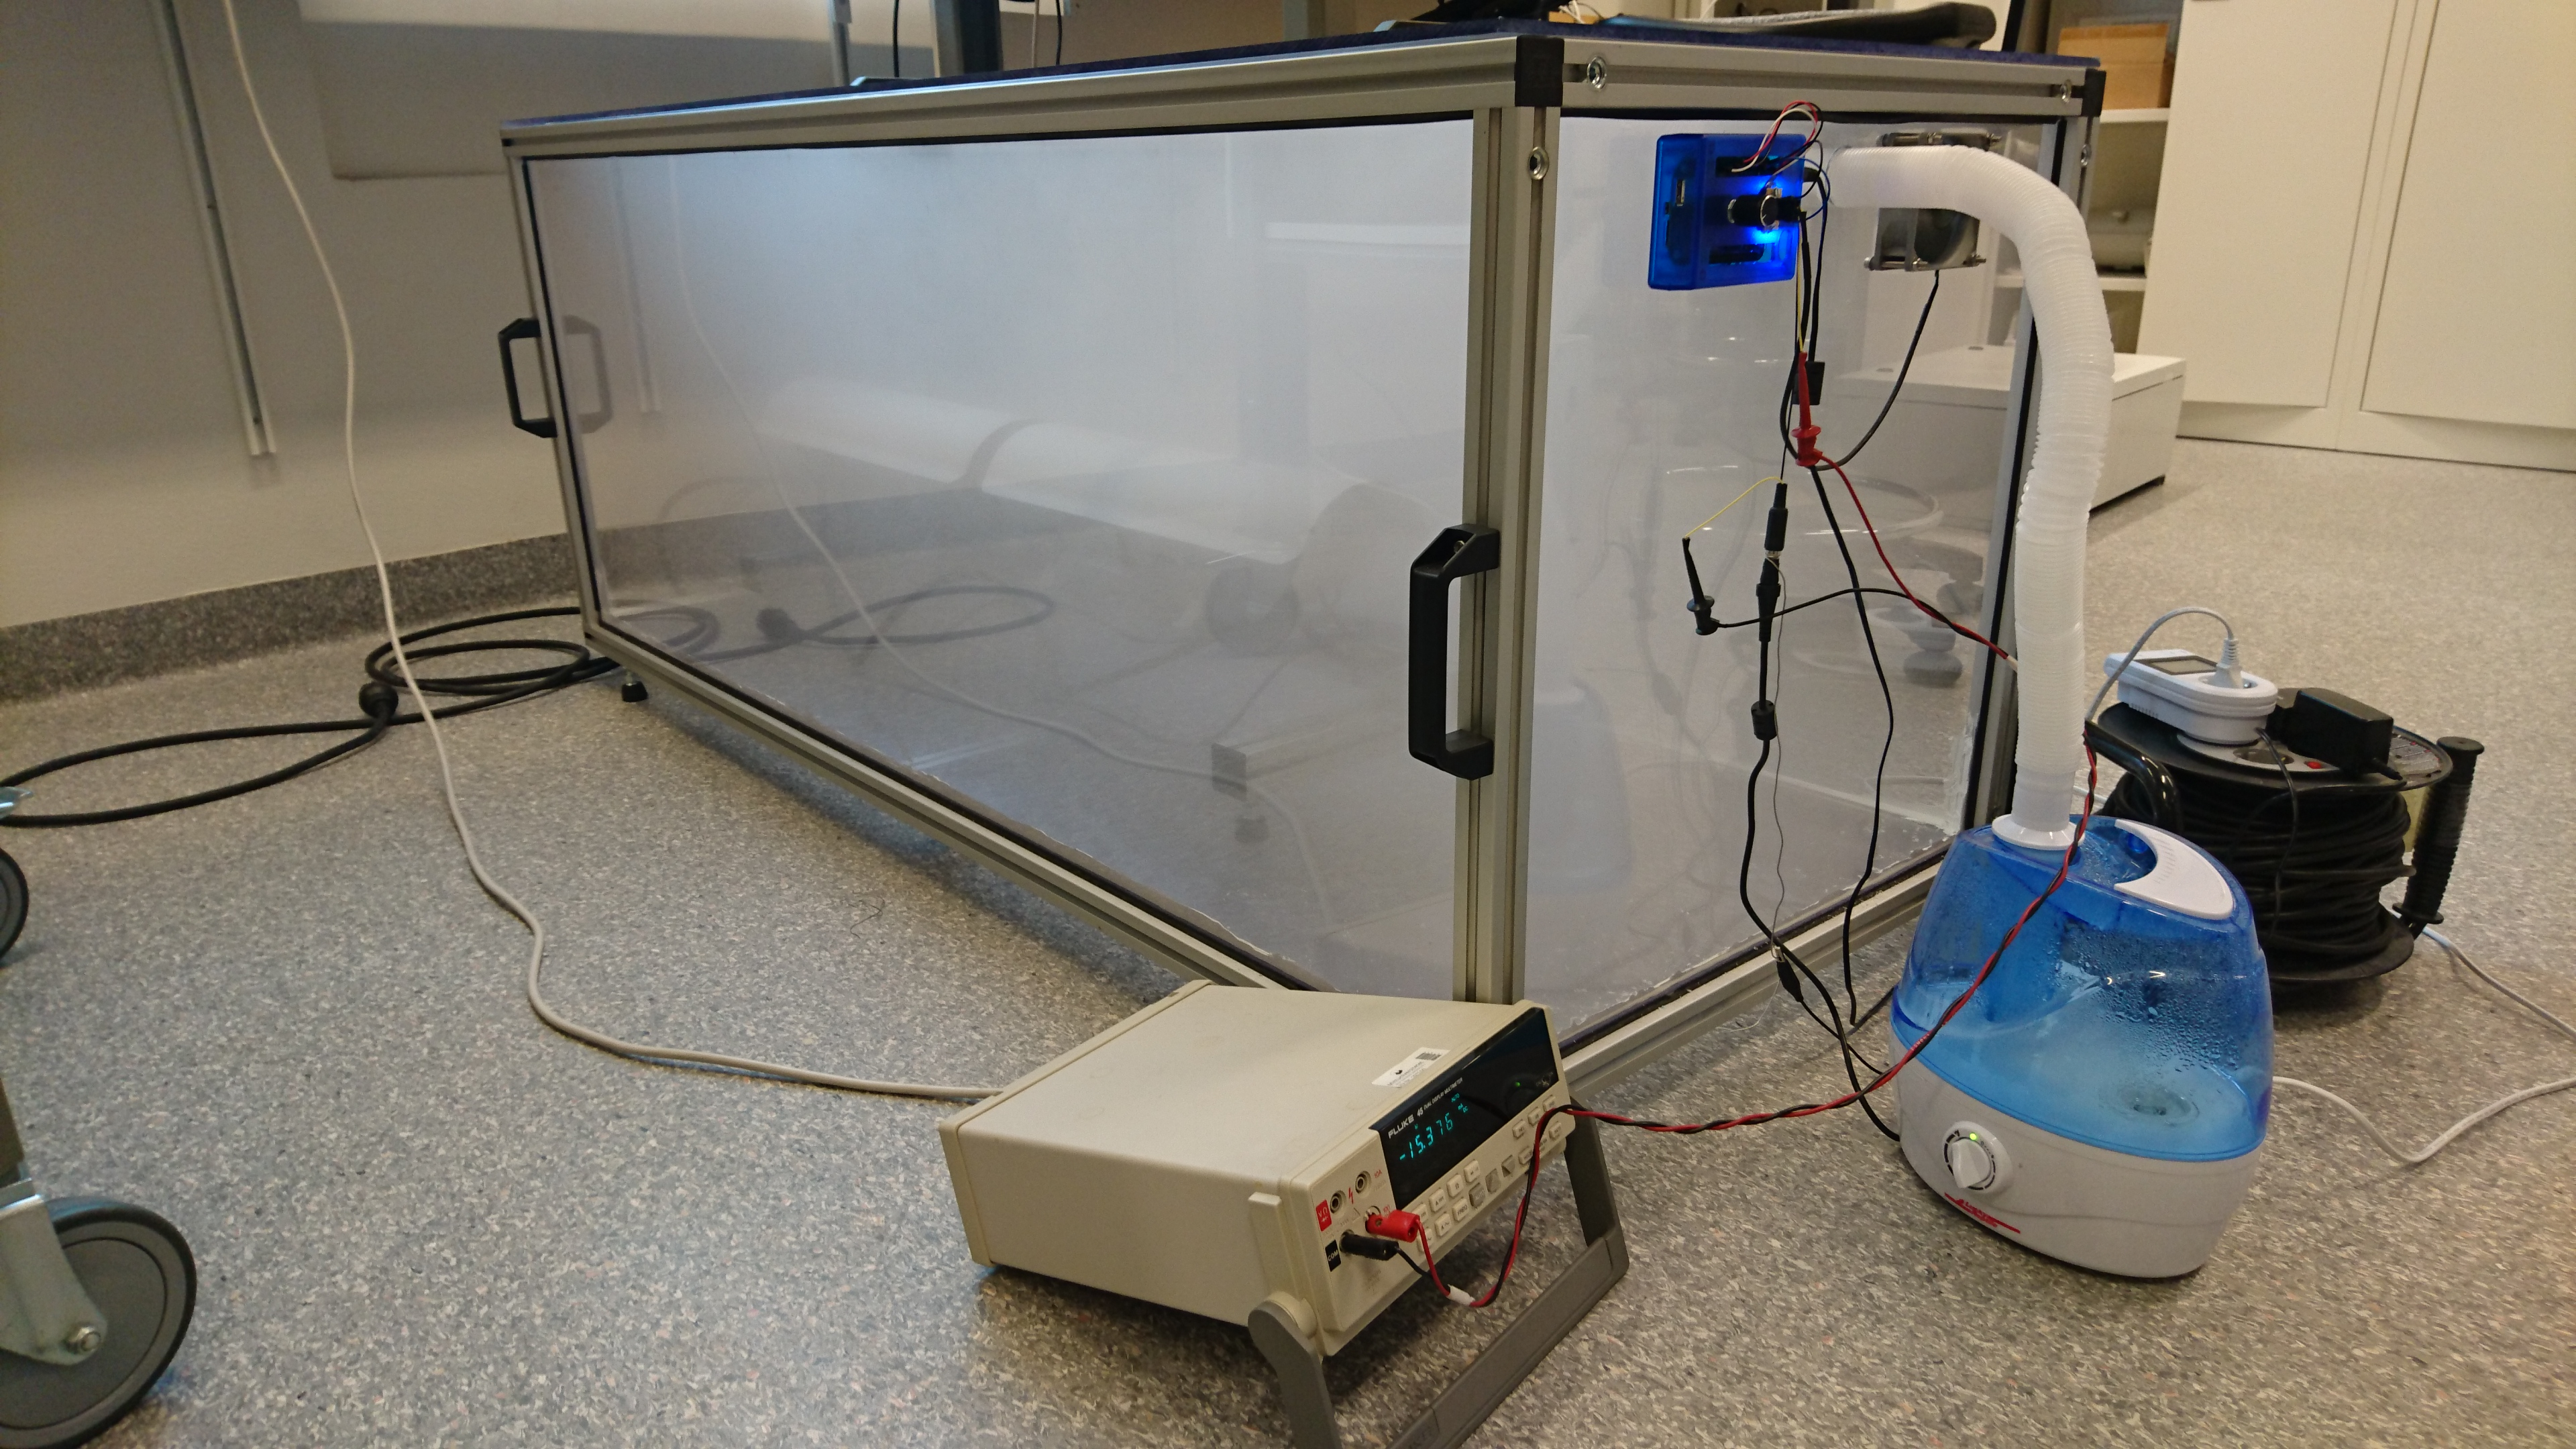
\includegraphics[width=0.6\linewidth]{figures/DSC_0103}
\caption{Fog chamber with connected droplet generator (blue container) and a multimeter used for fan power measurement. A Beaglebone Black microcontroller (blue box) is used for fan speed regulation.}
\end{figure}





\begin{equation}
E^{\prime} = \hbar\omega^{\prime} = \frac{\hbar\omega}{1+ \frac{\hbar\omega}{m_{e}c^{2}}\left(1-\cos\theta\right)}
\end{equation} 


%\begin{figure}[h]
%	\centering
%	\subfloat[Photoelectric effect]{\inputtikz{0.44}{photoelectric_effect.pgf}\label{fig:photoeffect}}
%	\subfloat[Compton effect]{\inputtikz{0.4}{compton_effect.pgf}\label{fig:compton}}
%	\caption[Processes of the photoelectric effect (a) and Compton effect (b).]{Sketch showing the processes of the photoelectric effect (a) and Compton effect (b).}
%\end{figure}

\section{Hybrid pixel detectors}
\Cref{fig:pixel_matrix} shows a hybrid pixel detector.\todocite{Medipix paper}
%\begin{figure}[ht]
%    \centering
%    \hspace{1cm}
%    \inputtikz{0.75}{pixel_detector.pgf}
%    \caption[Sketch of a hybrid pixel detector.]{Sketch of a hybrid pixel detector. The chip contains amplifiers and pixel logic as well as controlling periphery. Solder bumps are placed on the bump pads on the chip and pressed against their counterpart on the sensor.}
%    \label{fig:pixel_matrix}
%\end{figure}
\todo[inline]{Rember to write more text here...}
% this is shows the paper size and measures
%\begin{figure}
%    \oddpagelayouttrue
%    \twocolumnlayoutfalse
%    \stockdiagram
%    \caption{Right-hand page major layout parameters for
%        the \file{memoir} class} \label{fig:mempplt}
%\end{figure}
%\stockvalues